% !Mode:: "TeX:UTF-8"
% !TEX root = hnumain.tex

\iffalse
\bibliography{reference/reference.bib} % 欺骗latextools获取bib文件
\fi

%%%%%%% 正文 %%%%%%%
\chapter{绪论}

\section{研究背景和意义}

番木瓜（\textit{Carica papaya} L.）因其果实口感丰富、香气浓郁并且具有显著的药用价值而备受推崇\cite{liudifa2023papaya}。
番木瓜在食品、药品及化妆品等领域的需求日益增加，例如番木瓜蛋白酶的就呈现出供不应求的局面\cite{huangqiulan2022enzyme}。在2010年到
2021年的10年间，全国番木瓜种植面积已经从7601公顷增长到10680公顷\cite{chenyan2024germplasm}。

\section{国内外研究现状}
机器视觉技术凭借自身所具有的非破坏性、高效以及准确等特性，已然在农业智能化领域得到了广泛应用\cite{shin2022machinevision}，而且还有诸多针对果实成熟度判别方面的解决方案。

\chapter{材料与方法}
\section{数据采集及处理}
\subsection{图像采集}
实验所用的番木瓜图像主要来自线下果园拍摄和网络公开数据集。实验地点为海南大学儋州校区新农科基地（19.50°N, 109.48°E），该实验基地内有一番木瓜果园，内共种植约150株番木瓜。本次实验拍摄的番木瓜于8月坐果，到12月陆续成熟。

\begin{figure}[h]
\centering
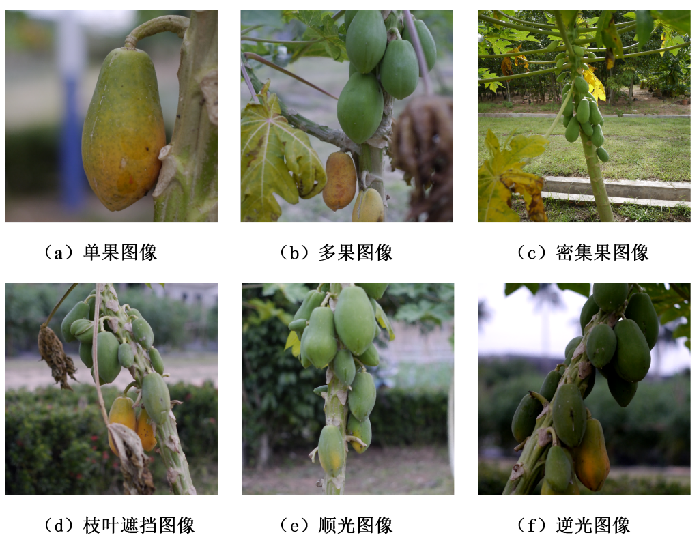
\includegraphics[width=0.75\textwidth]{figures/fig2-1.pdf}
\caption{番木瓜果园采集图像示例}\label{fig:fig2-1}
\vspace{-1em}
\end{figure}


\section{试验环境}


其他网络超参数如表\ref{tab:table2-2}所示。
\begin{table}[h]
    \caption{YOLOv11网络超参数}\label{tab:table2-2}
    \vspace{0.5em}\centering\wuhao
    \begin{tabular}{ll}
    \toprule[1.5pt]
    Hyperparameter & Value \\
    \midrule[1pt]
    每批次图像数量(batch) & 72 \\
    训练轮次(epoch) & 250 \\
    输入图像尺寸(image size) & 640 \\
    动量(momentum) & 0.973 \\
    初始学习率(lr0) & 0.01 \\
    最终学习率(lrf) & 0.01 \\
    权重衰减(weight\_decay) & 0.005 \\
    \bottomrule[1.5pt]
    \end{tabular}
    \vspace{\baselineskip}
    \end{table}

\section{模型评价指标}
计算公式：

（1）准确率：

\begin{equation}
\label{eq:precision}
\mathrm{Precision} = \frac{TP}{TP + FP}
\end{equation}

（2）召回率：
\begin{equation}
\label{eq:recall}
\mathrm{Recall} = \frac{TP}{TP + FN}
\end{equation}


\chapter{结果与分析}
\section{模型改进结果}
这是模型改进结果部分的内容。


\chapter{结论}
这是结论部分的内容。

